\FILE{section-nlp.tex}

\section{NLP}


Natural Language Processing was one of the first services offered by
many cloud providers. This was motivated by analyzing large amounts of
text in volume and number and deriving automated content from
it. Popular services include keyword extraction, sentiment analysis,
auto summary, and translation.  The services are offered often by large
cloud providers such as Google, IBM Watson and Amazon to consumers for
a fee. In addition such tools are also offered as stand alone
components and software packages.

As many such services are offered by the different providers, and
standalone components and software packages exist, it allows us to use
them to test the framework for implementing hybrid and multi-cloud
analytics services. We can therefore analyze each of their APIs and
compare functionality as well as the performance characteristics of
local as well as cloudservices. We also can test our design of the
cloud service catalog to identify the strategy of dynamically
locating similar services and integrate them into a service offering.

For our work we have restricted our analysis to two cloud services
from Amazon ans Google, while the integration of a third from Amazon
is under development. Furthermore we have only considered the
translation service as it provides an easy abstraction of a service
that translates a text from a source language to a target langauge:

\begin{Verbatim}[fontsize=\small]
def translate(text, source_langauge, target_langauage, ...):
    ...
    return translation
\end{Verbatim}

Each of the services is implemented with a different API. We contrast
the API in Figure ... showcaseing the difference in invoking a
translation service as well as showcasing the result of the json
response of such a service.


If the interface is on purpose defined differently a switch will cost
extra work and may therfore not be in the interest of the users.  It
is obvious that users can benefit from a uniform implementation of
this API in order to easily switch from one provider to the other.
Naturally the cloud providers typically do not have any interrest in
providing such a uniform API as it may entise the customers to switch
service providers.

Hence a multicloud CLI implementation may look as followes, where the
provider flag is used to distinguish the different cloud providers
offering the translation service. Naturally, we could also utilize a
local translation program such as offered from ... and easily make
this example a hybrid service that also integrates with a local
implementation.


\begin{Verbatim}[fontsize=\small]
cms nlp translate --provider=google --from=en --to=de hello world
cms nlp translate --provider=aws --from=en --to=de hello world
cms nlp translate --provider=local --from=en --to=de hello world
\end{Verbatim}


As eachof the services returns natively a different outout, it is
beneficial to unify the output and create a mapping from the
originating service to the output. An example for such a uniform output is given next.
ml          

\begin{Verbatim}[fontsize=\small]
{'date': '05/02/2022 14:45:45',
 'input': 'hello world',
 'input_language': 'en',
 'output': 'Hallo Welt',
 'output_language': 'de',
 'provider': 'aws',
 'time': 0.2641}
\end{Verbatim}


Other parameters such as service region can easily be integrated in
this example. Furthermore, it is obvious that the commandline
application underlaying API can be used in a REST service
implementation and can be generalized into different REST service
frameworks. For our implementation we have used FastAPI and used the
closest regional service center to our location.

The result of the translation that simply translates a text from
German ``Hallo Welt'' to English ``Hello World'' is showcased for 100
invocations in Figure~\ref{fig:translate}. 

\begin{figure}[htb]
  \begin{center}
    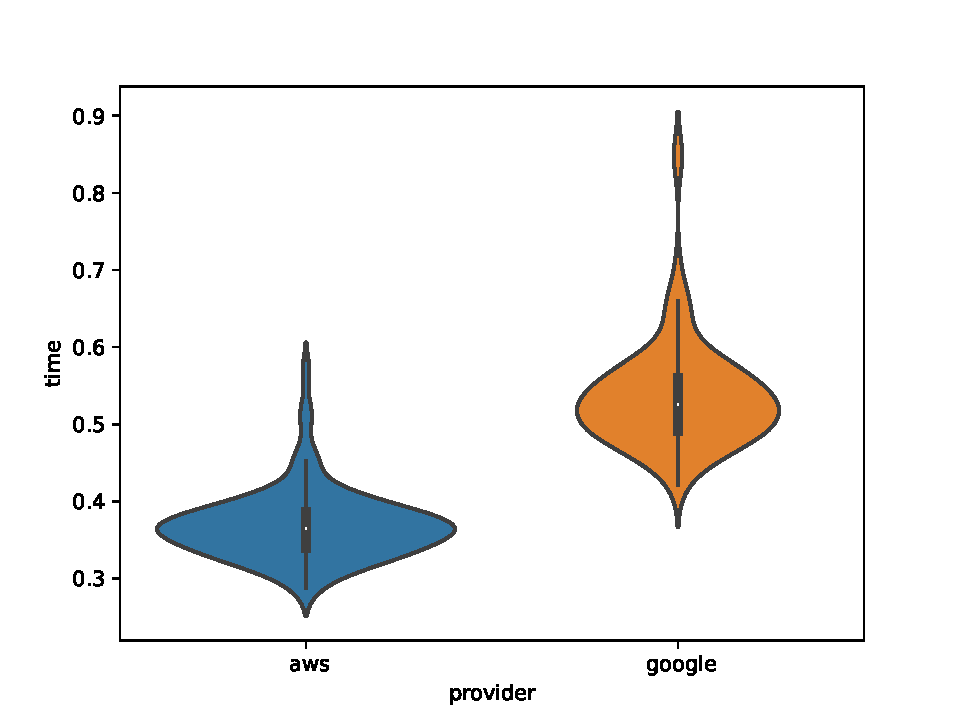
\includegraphics[width=1.0\columnwidth]{images/nlp-helloworldbenchmark.pdf}
    \end{center}
  \caption {Architecture of the hybrid multi-analytics service
    framework}
  \label{fig:translate}
\end{figure}

Such a performance analysis could be performed based on customer needs
and could indicate factors for preferential service choices. THis may
include besides time other factors such as cost and qaulity, or even
service level reliability at different times.

For us we found that in for the short query we used the service
offered by AWS to translate the text was on average ...  seconds
faster when executed from Bloomington, IN to the closest service
centers for the providor.



